\chapter{Analisis}
\label{chap: analisis}

\section{Analisis Sistem Kini}
\label{sec: analisiSKini}

Analisis sistem kini akan menjelaskan bagaimana sistem penilaian sidang skripsi 2 yang telah ada dan dipakai pada saat ini di Universitas Katolik Parahyangan jurusan Teknik Informatika. Berikut ini adalah penjelasan penggunaan kertas \textit{form} tersebut:

	\subsection{Form Rekapitulasi Penilaian}
	\label{sub: rekapPenil}
	
	\textit{Form} rekapitulasi dibagi menjadi 3 bagian(Gambar\ref{fig: rekapAsli}), yaitu:
		\begin{enumerate}
			\item Lembar Rekapitulasi Penilaian Pembimbing
			\item Lembar Rekapitulasi Penilaian Ketua Tim Penguji
			\item Lembar Rekapitulasi Penilaian Anggota Tim Penguji
		\end{enumerate}
	
	Ketiga lembaran tersebut akan dipotong dan diberikan kepada pembimbing, ketua tim penguji, dan anggota tim penguji sesuai dengan keperluannya. Setelah dibagikan, penilai wajib mengisi kolom nilai yang ingin diberikan kepada mahasiswa yang bersangkutan sesuai dengan kolom komponen penilaian yang ada. Setelah penilai memberikan nilai, maka penilai harus melakukan perkalian antara kolom nilai dengan kolom bobot yang akan menghasilkan kolom nilai akhir mahasiswa. Terakhir penilai akan menjumlahkan seluruh kolom nilai akhir yang akan menghasilkan total nilai akhir dari mahasiswa tersebut.
	
	Setelah semua kolom terisi, maka lembaran rekapitulasi tersebut akan dikumpulkan ke ketua tim penguji. Kemudian data yang telah tersedia akan disalin oleh ketua tim penguji kepada \textit{form} berita acara sidang skripsi.
	
	\subsection{Form Berita Acara Sidang Skripsi}
	\label{sub: formSkripsi}
	
	\textit{Form} berita acara sidang skripsi merupakan \textit{form} yang mencakup pengisian waktu sidang bersangkutan, data diri mahasiswa, nama dosen penguji dan pembimbing, nilai akhir dari masing-masing penilai, dan nilai akhir yang diterima mahasiswa. Seperti yang telah dibahas pada subbab sebelumnya(\ref{sub: rekapPenil}) \textit{form} berita acara sidang skripsi akan diisi oleh ketua tim penguji setelah seluruh form rekapitulasi dari masing masing penilai di kumpulkan kembali kepada ketua tim penguji.
	
	Setelah ketua tim penguji melakukan pengisian pada masing-masing kolom nilai dari masing-masing penilai yang bersangkutan, maka ketua tim penguji akan melakukan perkalian nilai tersebut dengan bobot masing-masing penilai yang akan menghasilkan nilai akhir mahasiswa dari masing-masing penilai. Kemudian akan dihasilkan 90\% nilai akhir mahasiswa untuk diberitahukan kepada mahasiswa dan diberikan kepada koordinator skripsi untuk melengkapi 10\% dari nilai mahasiswa berdasarkan nilai kedisiplinan. Hasil dari seluruh proses tersebut adalah nilai akhir sidang skripsi 2 mahasiswa bersangkutan.
	
\section{Analisis Sistem Usulan}
\label{sec: analisisSUsulan}

Analisis sistem usulan dibagi menjadi beberapa tahap, yaitu analisis \textit{back end}, analisis \textit{front end}, dan analisis basis data. Berikut ini penjelasannya:
	
	\subsection{Analisis Back End}
	\label{sub: backEnd}
	
	Analisis tahap \textit{back end} merupakan analisis pada lapisan data akses dan kode-kode yang bekerja secara tidak terlihat pada suatu aplikasi. Pada sistem informasi penilaian sidang skripsi 2, analisis tahap ini membahas tentang pembuatan kode \textit{model, view, controller} dari \textit{codeigniter}. Berikut ini adalah penjelasan lengkapnya:
	
	\subsubsection{Model}
	\label{subsub: modelCI}
	
	Pada bagian ini akan dijelaskan tentang penggunaan \textit{model} pada \textit{codeigniter}. \textit{Model} mempunyai fungsi untuk membuat sambungan dari aplikasi ke basis data. Pada \textit{codeigniter} pemanggilan \textit{model} dilakukan pada file \textit{controller} dengan menggunakan fungsi khusus \textit{codeigniter} yaitu:
	\begin{lstlisting}
	$data = $this->skripsi_model->getAllMahasiswa();
	\end{lstlisting}
	
	Kode di atas merupakan fungsi dari \textit{codeigniter} yang melakukan pemanggilan terhadap \textit{file model} yang akan dipakai. Pada kasus sistem usulan, nama \textit{file model} yang digunakan adalah "skripsi\_model". \textit{Model} sendiri berisi kode-kode sebagai berikut:
	\begin{lstlisting}
		<?php
		defined('BASEPATH') OR exit('No direct script access allowed');
		
		class Skripsi_model extends CI_Model {
		
			public function insertDataMahasiswa($tableName, $data){
				$res = $this->db->insert($tableName, $data);
			}
		}
	\end{lstlisting}
	
	Berikut adalah \textit{method} yang dimiliki oleh kelas \textit{model}:
	\begin{itemize}
		\item public function insertDataMahasiswa(\$tablename, \$data)\\
		Berfungsi untuk melakukan fungsi \textit{insert} pada basis data.\\
		Parameter: 
		\begin{itemize}
			\item tablename merepresentasikan nama tabel basis data.
			\item data merepresentasikan data dari controller yang sudah diubah dan ingin dimasukkan kedalam basis data.
		\end{itemize}
	\end{itemize}
	
	\subsubsection{Controller}
	\label{subsub: controllerCI}
	
	Pada bagian ini akan dijelaskan tentang kode dan kegunaannya pada kelas \textit{controller}. \textit{Controller} merupakan kelas yang mengatur hubungan antara kelas \textit{model} dan \textit{view} pada \textit{codeigniter}. Dengan memanfaatkan fungsi-fungsi dari \textit{codeigniter}, maka kelas \textit{controller} dapat dipersingkat dan dipermudah dalam pembuatannya. Berikut ini adalah kode pada kelas \textit{C\_Skripsi}:
\begin{lstlisting}
	<?php
	defined('BASEPATH') OR exit('No direct script access allowed');
	
	class C_skripsi extends CI_Controller {
	
	/**
	* Index Page for this controller.
	*
	* Maps to the following URL
	*              http://example.com/index.php/welcome
	*      - or -
	*              http://example.com/index.php/welcome/index
	*      - or -
	* Since this controller is set as the default controller in
	* config/routes.php, it's displayed at http://example.com/
	*
	* So any other public methods not prefixed with an underscore will
	* map to /index.php/welcome/<method_name>
	* @see https://codeigniter.com/user_guide/general/urls.html
	*/
		public function index()
		{
			$this->load->view('skripsi');
		}
		//Check database
		public function view_cekMahasiswa(){
			$data = $this->skripsi_model->getAllMahasiswa();
			$this->load->view('cek_mahasiswa', array('data' => $data));
		}
		
		public function tambahDataMahasiswa(){
			$semester = $_POST['semester'];
			$tahun = $_POST['tahun'];
			$npm = $_POST['npm'];
			$nama = $_POST['nama'];
			$judul = $_POST['judul'];
			$namaPembimbing = $_POST['namaPembimbing'];
			$namaPembimbingPendamping = $_POST['namaPembimbingPendamping'];
			$namaKetuaTimPenguji = $_POST['namaKetuaTimPenguji'];
			$namaAnggotaTimPenguji = $_POST['namaAnggotaTimPenguji'];
			$bobotKetuaTimPenguji = $_POST['bobotKetuaTimPenguji'];
			$bobotAnggotaTimPenguji = $_POST['bobotAnggotaTimPenguji'];
			$bobotPembimbing = $_POST['bobotPembimbing'];
			$nilaiKoordinatorSkripsi = $_POST['nilaiKoordinatorSkripsi'];
			$bobotKoordinatorSkripsi = $_POST['bobotKoordinatorSkripsi'];
			$bobotTataTulisLaporanAnggota = $_POST['bobotTataTulisLaporanAnggota'];
			$bobotKelengkapanMateriAnggota = $_POST['bobotKelengkapanMateriAnggota'];
			$bobotPenguasaanMateriAnggota = $_POST['bobotPenguasaanMateriAnggota'];
			$bobotPresentasiAnggota = $_POST['bobotPresentasiAnggota'];
			$bobotPencapaianTujuanAnggota = $_POST['bobotPencapaianTujuanAnggota'];
			$bobotTataTulisLaporanKetua = $_POST['bobotTataTulisLaporanKetua'];
			$bobotKelengkapanMateriKetua = $_POST['bobotKelengkapanMateriKetua'];
			$bobotPenguasaanMateriKetua = $_POST['bobotPenguasaanMateriKetua'];
			$bobotPresentasiKetua = $_POST['bobotPresentasiKetua'];
			$bobotPencapaianTujuanKetua = $_POST['bobotPencapaianTujuanKetua'];
			$bobotTataTulisLaporanPembimbing = $_POST['bobotTataTulisLaporanPembimbing'];
			$bobotKelengkapanMateriPembimbing = $_POST['bobotKelengkapanMateriPembimbing'];
			$bobotPenguasaanMateriPembimbing = $_POST['bobotPenguasaanMateriPembimbing'];
			$prosesBimbinganPembimbing = $_POST['prosesBimbinganPembimbing'];
			$nilaiAkhirMahasiswa = $_POST['nilaiAkhirMahasiswa'];
			$data_insert = array(
				'semester' => $semester,
				'tahun' => $tahun,
				'npm' => $npm,
				'nama' => $nama,
				'judul' => $judul,
				'namaPembimbing' => $namaPembimbing,
				'namaPembimbingPendamping' => $namaPembimbingPendamping,
				'namaKetuaTimPenguji' => $namaKetuaTimPenguji,
				'namaAnggotaTimPenguji' => $namaAnggotaTimPenguji,
				'bobotKetuaTimPenguji' => $bobotKetuaTimPenguji,
				'bobotAnggotaTimPenguji' => $bobotAnggotaTimPenguji,
				'bobotPembimbing' => $bobotPembimbing,
				'nilaiKoordinatorSkripsi' => $nilaiKoordinatorSkripsi,
				'bobotKoordinatorSkripsi' =>$bobotKoordinatorSkripsi,
				'bobotTataTulisLaporanAnggota' => $bobotTataTulisLaporanAnggota,
				'bobotKelengkapanMateriAnggota' => $bobotKelengkapanMateriAnggota,
				'bobotPenguasaanMateriAnggota' => $bobotPenguasaanMateriAnggota,
				'bobotPresentasiAnggota' => $bobotPresentasiAnggota,
				'bobotPencapaianTujuanAnggota' => $bobotPencapaianTujuanAnggota,
				'bobotTataTulisLaporanKetua' => $bobotTataTulisLaporanKetua,
				'bobotKelengkapanMateriKetua' => $bobotKelengkapanMateriKetua,
				'bobotPenguasaanMateriKetua' => $bobotPenguasaanMateriKetua,
				'bobotPresentasiKetua' => $bobotPresentasiKetua,
				'bobotPencapaianTujuanKetua' => $bobotPencapaianTujuanKetua,
				'bobotTataTulisLaporanPembimbing' => $bobotTataTulisLaporanPembimbing,
				'bobotKelengkapanMateriPembimbing' => $bobotKelengkapanMateriPembimbing,
				'bobotPenguasaanMateriPembimbing' => $bobotPenguasaanMateriPembimbing,
				'prosesBimbinganPembimbing' => $prosesBimbinganPembimbing,
				'nilaiAkhirMahasiswa' => $nilaiAkhirMahasiswa,
			
			);
			$res = $this->skripsi_model->insertDataMahasiswa('beritaacarasidangskripsi',$data_insert);
			redirect(base_url(), 'refresh');
		}
	
	}
	
\end{lstlisting}

Berikut adalah \textit{method-method} yang dimiliki oleh kelas \textit{controller}:
\begin{itemize}
	\item view\_cekMahasiswa\\
	Berfungsi untuk memilih \textit{file view} dan \textit{model} yang akan dipakai pada sistem informasi.
	\item tambahDataMahasiswa\\
	Berfungsi untuk mengambil data yang telah terisi dari \textit{view} sistem dan mengubahnya menjadi \textit{compatible} sehingga dapat diproses kedalam \textit{method} insertDataMahasiswa pada kelas \textit{model} yang kemudian akan diproses ke dalam bahasa sql.
\end{itemize}
	
	\subsection{Analisis Front End}
	\label{sub: frontEnd}
	
	Pada subbab ini akan dijelaskan bagaimana pembuatan dan fungsi otomatisasi dari AngularJS di sistem usulan. Berikut ini adalah contoh proses otomatisasi pada sistem usulan:
	
\begin{lstlisting}
<body ng-app="penilaian">
	<form ng-controller="DefaultValue">
	
	</form>
	
	<script>
	angular.module('penilaian', [])
	.controller('DefaultValue', ['$scope', function ($scope) {
	
	}]);
	</script>
</body>
\end{lstlisting}
	`
	
	Contoh diatas adalah inisialisasi dari AngularJS dengan menggunakan fungsi ng-app dan ng-controller yang mengatur keseluruhan fungsi otomatisasi pada sistem usulan. Pada baris pertama dilakukan inisialisasi ng-app yang berfungsi menginisialisasi nama app yang digunakan pada sistem. Setelah ng-app diinisialisasi, baru sistem usulan dapat menggunakan fungsi-fungsi AngularJS seperti menginisialisasi ng-controller pada baris ke-2 dengan nama "Default Value".\\
	Agar \textit{controller} dapat berfungsi, perlu dilakukan pemanggilan terhadap ng-controller dengan memanfaatkan fungsi "angular.module". Baris ke-7 bekerja dengan \textit{parameter} ng-app("penilaian"). Selanjutnya diikuti dengan sebuah \textit{array}(\[\]) kosong yang merupakan tempat yang menunjukkan \textit{list modules} diperlukan oleh ng-app('penilaian') Setelah melakukan inisialisasi modul, maka kita dapat memanggil fungsi-fungsi daripada AngularJS untuk dijalankan, seperti \textit{controller("DefaultValue")} ke dalam aplikasi AngularJS.
	
\begin{lstlisting}
<tr>
	<td><label for="nTTLaporanK">Tata Tulis Laporan</label></td>
	<td><input type="number" id="nTTLaporanK" max="100" ng-model="nilai_TTLaporanK" class="form-nilai"/></td>
	<!-- 20 -->
	<td><input type="number" name="bobotTataTulisLaporanKetua" ng-model="TTLaporanK.value" ng-init="TTLaporanK.value = 15" min="0" max="100" class="form-nilai" readonly="readonly" /></td>
	<td><input type="number" disabled="disabled" value="{{nilai_TTLaporanK * TTLaporanK.value / 100}}" ng-model="total_TTLaporanK" class="form-nilai"/></td>
</tr>
\end{lstlisting}
	
	Contoh diatas diambil dari kode \textit{file view} untuk mengatur otomatisasi pada kolom tata tulis laporan milik ketua tim penguji. Pada baris ke-3 dan baris ke-5 adalah contoh kode diatas merupakan contoh inisialisasi fungsi ng-model dari AngularJS, sementar baris ke-6 dilakukan perhitungan otomatis dari ng-model baris ke-3 dikalikan dengan ng-model baris ke-5 dan hasilnya ditampung di nilai \textit{value} yang kemudian akan muncul ke layar \textit{user} secara otomatis.
	
	Berikut ini adalah nama-nama dari \textit{model, view,} dan \textit{controller} AngularJS yang dipakai pada sistem penilaian sidang skripsi 2:
	\begin{itemize}
		\item \textit{Controller}: "DevaultValue" = Controller yang dipakai di seluruh sistem
		\item \textit{Model}:
		\begin{itemize}
			\item "tahun" = untuk melakukan otomatisasi tahun+1
			\item "n\_npm" = untuk melakukan pengisian otomatis npm mahasiswa pada smua lembaran penilaian
			\item "nilai\_ketua" = untuk menyimpan hasil perolehan total nilai dari lembar rekapitulasi ketua tim penguji
			\item "ketua.value" = untuk menyimpan bobot ketua tim penguji terhadap nilai akhir mahasiswa
			\item "total\_ketua" = untuk menyimpan perolehan nilai akhir dari ketua tim penguji
			\item "nilai\_anggota" = untuk menyimpan hasil perolehan total nilai dari lembar rekapitulasi anggota tim penguji
			\item "anggota.value" = untuk menyimpan bobot anggota tim penguji terhadap nilai akhir mahasiswa
			\item "total\_anggota" = untuk menyimpan perolehan nilai akhir dari anggota tim penguji
			\item "nilai\_pembimbing" = untuk menyimpan hasil perolehan total nilai dari lembar rekapitulasi pembimbing
			\item "pembimbing.value" = untuk menyimpan bobot pembimbing terhadap nilai akhir mahasiswa
			\item "total\_pembimbing" = untuk menyimpan perolehan nilai akhir dari pembimbing
			\item "nilai\_koordinator" = untuk menyimpan hasil perolehan total nilai dari lembar rekapitulasi koordinator
			\item "koodinator.value" = untuk menyimpan bobot koordinator terhadap nilai akhir mahasiswa
			\item "total\_koordinator" = untuk menyimpan perolehan nilai akhir dari koodinator
			\item "nilai\_TTLaporanK" = untuk menyimpan nilai tata tulis laporan pada lembar rekapitulasi ketua tim penguji
			\item "TTLaporanK.value" = untuk menyimpan bobot nilai tata tulis laporan pada lembar rekapitulasi ketua tim penguji
			\item "total\_TTLaporanK" = untuk menyimpan nilai akhir tata tulis laporan pada lembar rekapitulasi ketua tim penguji
			\item "nilai\_KMateriK" = untuk menyimpan nilai kelengkapan materi pada lembar rekapitulasi ketua tim penguji
			\item "KMateriK.value" = untuk menyimpan bobot nilai kelengkapan materi pada lembar rekapitulasi ketua tim penguji
			\item "total\_KMateriK" = untuk menyimpan bobot nilai akhir kelengkapan materi pada lembar rekapitulasi ketua tim penguji
			\item "nilai\_PMateriK" = untuk menyimpan nilai penguasaan materi pada lembar rekapitulasi ketua tim penguji
			\item "PMateriK.value" = untuk menyimpan bobot nilai penguasaan materi pada lembar rekapitulasi ketua tim penguji
			\item "total\_PMateriK" = untuk menyimpan bobot nilai akhir penguasaan materi pada lembar rekapitulasi ketua tim penguji
			\item "nilai\_presentasiK" = untuk menyimpan nilai presentasi pada lembar rekapitulasi ketua tim penguji
			\item "presentasiK.value" = untuk menyimpan bobot nilai presentasi pada lembar rekapitulasi ketua tim penguji
			\item "total\_presentasiK" = untuk menyimpan bobot nilai akhir presentasi pada lembar rekapitulasi ketua tim penguji
			\item "nilai\_PMateriK" = untuk menyimpan nilai penguasaan materi pada lembar rekapitulasi ketua tim penguji
			\item "PMateriK.value" = untuk menyimpan bobot nilai penguasaan materi pada lembar rekapitulasi ketua tim penguji
			\item "total\_PMateriK" = untuk menyimpan bobot nilai akhir penguasaan materi pada lembar rekapitulasi ketua tim penguji
			\item "nTotalKetua" = untuk menyimpan perhitungan nilai keseluruhan ketua tim penguji yang akan dimasukkan ke lembar berita acara sidang skripsi
			\item "nilai\_TTLaporanA" = untuk menyimpan nilai tata tulis laporan pada lembar rekapitulasi anggota tim penguji
			\item "TTLaporanA.value" = untuk menyimpan bobot nilai tata tulis laporan pada lembar rekapitulasi anggota tim penguji
			\item "total\_TTLaporanA" = untuk menyimpan nilai akhir tata tulis laporan pada lembar rekapitulasi anggota tim penguji
			\item "nilai\_KMateriA" = untuk menyimpan nilai kelengkapan materi pada lembar rekapitulasi anggota tim penguji
			\item "KMateriA.value" = untuk menyimpan bobot nilai kelengkapan materi pada lembar rekapitulasi anggota tim penguji
			\item "total\_KMateriA" = untuk menyimpan bobot nilai akhir kelengkapan materi pada lembar rekapitulasi anggota tim penguji
			\item "nilai\_PMateriA" = untuk menyimpan nilai penguasaan materi pada lembar rekapitulasi anggota tim penguji
			\item "PMateriA.value" = untuk menyimpan bobot nilai penguasaan materi pada lembar rekapitulasi anggota tim penguji
			\item "total\_PMateriA" = untuk menyimpan bobot nilai akhir penguasaan materi pada lembar rekapitulasi anggota tim penguji
			\item "nilai\_presentasiA" = untuk menyimpan nilai presentasi pada lembar rekapitulasi anggota tim penguji
			\item "presentasiA.value" = untuk menyimpan bobot nilai presentasi pada lembar rekapitulasi anggota tim penguji
			\item "total\_presentasiA" = untuk menyimpan bobot nilai akhir presentasi pada lembar rekapitulasi anggota tim penguji
			\item "nilai\_PMateriA" = untuk menyimpan nilai penguasaan materi pada lembar rekapitulasi anggota tim penguji
			\item "PMateriA.value" = untuk menyimpan bobot nilai penguasaan materi pada lembar rekapitulasi anggota tim penguji
			\item "total\_PMateriA" = untuk menyimpan bobot nilai akhir penguasaan materi pada lembar rekapitulasi anggota tim penguji
			\item "nTotalAnggota" = untuk menyimpan perhitungan nilai keseluruhan anggota tim penguji yang akan dimasukkan ke lembar berita acara sidang skripsi
			\item "nilai\_TTLaporanP" = untuk menyimpan nilai tata tulis laporan pada lembar rekapitulasi pembimbing tim penguji
			\item "TTLaporanP.value" = untuk menyimpan bobot nilai tata tulis laporan pada lembar rekapitulasi pembimbing
			\item "total\_TTLaporanP" = untuk menyimpan nilai akhir tata tulis laporan pada lembar rekapitulasi pembimbing
			\item "nilai\_KMateriP" = untuk menyimpan nilai kelengkapan materi pada lembar rekapitulasi pembimbing
			\item "KMateriP.value" = untuk menyimpan bobot nilai kelengkapan materi pada lembar rekapitulasi pembimbing
			\item "total\_KMateriP" = untuk menyimpan bobot nilai akhir kelengkapan materi pada lembar rekapitulasi pembimbing
			\item "nilai\_PMateriP" = untuk menyimpan nilai penguasaan materi pada lembar rekapitulasi pembimbing
			\item "PMateriP.value" = untuk menyimpan bobot nilai penguasaan materi pada lembar rekapitulasi pembimbing
			\item "total\_PMateriP" = untuk menyimpan bobot nilai akhir penguasaan materi pada lembar rekapitulasi pembimbing
			\item "nilai\_PBimbinganP" = untuk menyimpan nilai proses bimbingan pada lembar rekapitulasi pembimbing
			\item "PBimbinganP.value" = untuk menyimpan bobot nilai proses bimbingan pada lembar rekapitulasi pembimbing
			\item "total\_PBimbinganP" = untuk menyimpan bobot nilai akhir proses bimbingan pada lembar rekapitulasi pembimbing
			\item "nTotalPembimbing" = untuk menyimpan perhitungan nilai keseluruhan pembimbing yang akan dimasukkan ke lembar berita acara sidang skripsi
		\end{itemize}
		\item View:
		\begin{itemize}
			\item "\{\{tahun+1\}\}" = menampilkan hasil dari model "tahun" ditambahkan dengan 1
			\item "\{\{ n\_npm \}\}" = menampilkan npm mahasiswa
			\item \{\{nilai\_TTLaporanK * TTLaporanK.value / 100 + nilai\_KMateriK * KMateriK.value / 100 + nilai\_PMateriK * PMateriK.value / 100 + nilai\_PresentasiK * presentasiK.value / 100 + nilai\_PTujuanK * PTujuanK.value / 100\}\}" = nilai ketua tim penguji pada lembar berita acara sidang skripsi
			\item "\{\{(nilai\_TTLaporanK * TTLaporanK.value / 100 + nilai\_KMateriK * KMateriK.value / 100 + nilai\_PMateriK * PMateriK.value / 100 + nilai\_PresentasiK * presentasiK.value / 100 + nilai\_PTujuanK * PTujuanK.value / 100) * ketua.value / 100\}\}" = menampilkan perhitungan nilai ketua dikalikan dengan bobot ketua tim penguji pada lembar berita acara sidang skripsi
			\item "\{\{nilai\_TTLaporanA * TTLaporanA.value / 100 + nilai\_KMateriA * KMateriA.value / 100 + nilai\_PMateriA * PMateriA.value / 100 + nilai\_PresentasiA * presentasiA.value / 100 + nilai\_PTujuanA * PTujuanA.value / 100\}\}" = nilai anggota tim penguji pada lembar berita acara sidang skripsi
			\item "\{\{(nilai\_TTLaporanA * TTLaporanA.value / 100 + nilai\_KMateriA * KMateriA.value / 100 + nilai\_PMateriA * PMateriA.value / 100 + nilai\_PresentasiA * presentasiA.value / 100 + nilai\_PTujuanA * PTujuanA.value / 100) * anggota.value / 100\}\}" = nilai anggota dikalikan dengan bobot anggota tim penguji pada lembar berita acara sidang skripsi
			\item "\{\{nilai\_TTLaporanP * TTLaporanP.value / 100 + nilai\_KMateriP * KMateriP.value / 100 + nilai\_PMateriP * PMateriP.value / 100 + nilai\_PBimbinganP * PBimbinganP.value / 100\}\}" = nilai pembimbing pada lembar berita acara sidang skripsi
			\item "\{\{(nilai\_TTLaporanP * TTLaporanP.value / 100 + nilai\_KMateriP * KMateriP.value / 100 + nilai\_PMateriP * PMateriP.value / 100 + nilai\_PBimbinganP * PBimbinganP.value / 100) * pembimbing.value / 100\}\}" = nilai pembimbing dikalikan bobot pembimbing pada lembar berita acara sidang skripsi
			\item "\{\{nilai\_koordinator*koordinator.value/100\}\}" = nilai koordinator skripsi dikalikan dengan bobot koordinator skripsi pada lembar berita acara sidang skripsi
			\item "\{\{ketua.value+anggota.value+pembimbing.value+koordinator.value\}\} = menampilkan total bobot pada lembar berita acara sidang skripsi
			\item "\{\{(nilai\_TTLaporanK * TTLaporanK.value / 100 + nilai\_KMateriK * KMateriK.value / 100 + nilai\_PMateriK * PMateriK.value / 100 + nilai\_PresentasiK * presentasiK.value / 100 + nilai\_PTujuanK * PTujuanK.value / 100 )* ketua.value / 100 + (nilai\_TTLaporanA * TTLaporanA.value / 100 + nilai\_KMateriA * KMateriA.value / 100 + nilai\_PMateriA * PMateriA.value / 100 + nilai\_PresentasiA * presentasiA.value / 100 + nilai\_PTujuanA * PTujuanA.value / 100) * anggota.value / 100 + (nilai\_TTLaporanP * TTLaporanP.value / 100 + nilai\_KMateriP * KMateriP.value / 100 + nilai\_PMateriP * PMateriP.value / 100 + nilai\_PBimbinganP * PBimbinganP.value / 100) * pembimbing.value / 100 + nilai\_koordinator * koordinator.value / 100\}\}" =  nilai akhir mahasiswa
			\item "\{\{nilai\_TTLaporanK * TTLaporanK.value / 100\}\}" = nilai tata tulis laporan ketua tim penguji
			\item "\{\{nilai\_KMateriK * KMateriK.value / 100 \}\}" =  nilai kelengkapan materi ketua tim penguji
			\item "\{\{nilai\_PMateriK * PMateriK.value / 100\}\}"  = nilai penguasaan materi ketua tim penguji
			\item "\{\{nilai\_PresentasiK * presentasiK.value / 100\}\}" = nilai presentasi ketua tim penguji
			\item "\{\{nilai\_PTujuanK * PTujuanK.value / 100\}\}" = nilai pencapaian tujuan ketua tim penguji
			\item "\{\{nilai\_TTLaporanK * TTLaporanK.value / 100 + nilai\_KMateriK * KMateriK.value / 100 + nilai\_PMateriK * PMateriK.value / 100 + nilai\_PresentasiK * presentasiK.value / 100 + nilai\_PTujuanK * PTujuanK.value / 100\}\}" = total nilai ketua tim penguji
			\item "\{\{nilai\_TTLaporanA * TTLaporanA.value / 100\}\}" = nilai tata tulis laporan anggota tim penguji
			\item "\{\{nilai\_KMateriA * KMateriA.value / 100\}\}" = nilai kelengkapan materi anggota tim penguji
			\item "\{\{nilai\_PMateriA * PMateriA.value / 100\}\}" = nilai penguasaan materi ketua tim penguji
			\item "\{\{nilai\_PresentasiA * presentasiA.value / 100\}\}" = nilai presentasi anggota tim penguji
			\item "\{\{nilai\_PTujuanA * PTujuanA.value / 100\}\}" = nilai pencapaian tujuan anggota tim penguji
			\item "\{\{nilai\_TTLaporanA * TTLaporanA.value / 100 + nilai\_KMateriA * KMateriA.value / 100 + nilai\_PMateriA * PMateriA.value / 100 + nilai\_PresentasiA * presentasiA.value / 100 + nilai\_PTujuanA * PTujuanA.value / 100\}\}" = total nilai anggota tim penguji
			\item "\{\{nilai\_TTLaporanP * TTLaporanP.value / 100\}\}" = nilai tata tulis laporan pembimbing
			\item "\{\{nilai\_KMateriP * KMateriP.value / 100\}\}" = nilai kelengkapan materi pembimbing
			\item "\{\{nilai\_PMateriP * PMateriP.value / 100\}\}" = nilai penguasaan materi pembimbing
			\item "\{\{nilai\_PBimbinganP * PBimbinganP.value / 100\}\}" = nilai proses bimbingan pembimbing
			\item "\{\{nilai\_TTLaporanP * TTLaporanP.value / 100 + nilai\_KMateriP * KMateriP.value / 100 + nilai\_PMateriP * PMateriP.value / 100 + nilai\_PBimbinganP * PBimbinganP.value / 100\}\}" = nilai akhir pembimbing
		\end{itemize}
	\end{itemize}
	
	\subsection{Analisis Basis Data}
	\label{sub: analisisDatabase}
	
	Sistem informasi penilaian sidang skripsi 2 menggunakan perangkat lunak mysql sebagai sarana penyimpanan dan pengolahan basis data. Seperti yang dijelaskan pada subbab \ref{sec: analisisKode}, didalam \textit{folder} "application" terdapat \textit{folder} "models" (Gambar\ref{fig:strukturFileApp}) yang berfungsi menghubungkan basis data dengan sistem. 
	
	Berdasarkan analisa dari contoh form penilaian skripsi yang ada (gambar \ref{fig: skripsiAsli} dan gambar \ref{fig: rekapAsli}), dapat disimpulkan bahwa penilaian skripsi membutuhkan data-data sebagai berikut:
		
		\begin{enumerate}
			\item Semester
			\item Tahun ajaran
			\item NPM mahasiswa 
			\item Nama mahasiswa
			\item Judul skripsi
			\item Nama pembimbing utama/tunggal
			\item Nama pembimbing pendamping(tidak harus)
			\item Nama ketua tim penguji
			\item Nama anggota tim penguji
			\item Bobot ketua tim penguji
			\item Bobot anggota tim penguji
			\item Bobot pembimbing
			\item Nilai koordinator skripsi
			\item Bobot koordinator skripsi
			\item Bobot tata tulis laporan ketua
			\item Bobot kelengkapan materi ketua
			\item Bobot penguasaan materi ketua
			\item Bobot presentasi ketua
			\item Bobot pencapaian tujuan ketua
			\item Bobot tata tulis laporan anggota
			\item Bobot kelengkapan materi anggota
			\item Bobot penguasaan materi anggota
			\item Bobot presentasi anggota
			\item Bobot pencapaian tujuan anggota
			\item Bobot tata tulis laporan pembimbing
			\item Bobot kelengkapan materi pembimbing
			\item Bobot penguasaan materi pembimbing
			\item Bobot bimbingan pembimbing
			\item Nilai akhir mahasiswa
		\end{enumerate}
	
	Berdasarkan diskusi dengan dosen pembimbing, disimpulkan bahwa sistem penilaian sidang skripsi 2 ini hanya memerlukan penyimpanan untuk bobot masing-masing penilaian dan nilai akhir mahasiswa untuk tahap perhitungan. Hal ini dikarenakan nilai-nilai lainnya dapat dihasilkan dengan melakukan perhitungan pada  nilai akhir mahasiswa dan bobot nilai yang diinginkan. Begitu pula dengan nilai dari masing-masing penguji.
	
\section{Use Case}
\label{sec: usecaseDiagram}

	\begin{figure}[H]
		\centering
		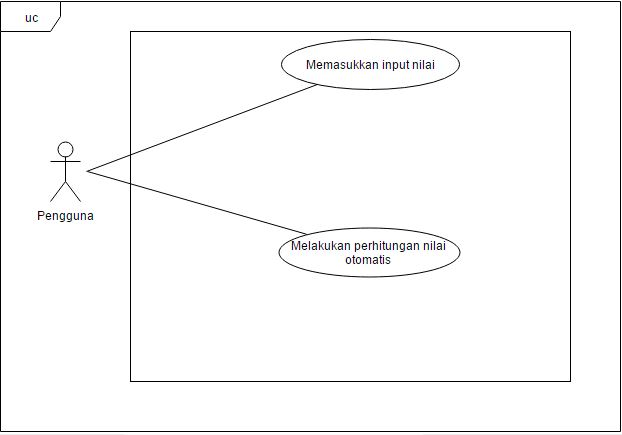
\includegraphics[scale=0.75]{Gambar/usecase}
		\caption{Use case diagram}
		\label{fig:usecase}
	\end{figure}
	
	\begin{enumerate}
		\item Skenario memasukkan nilai\\
			Deskripsi: Kegiatan memasukkan nilai ke dalam kotak input yang ada.\\
			Aktor: Pengguna\\
			Prakondisi: - \\
			Skenario:
			\begin{itemize}
				\item Pengguna memilih tempat/kolom yang sudah tersedia di tampilan
				\item Pengguna memasukkan nilai yang diinginkan pada tempat/kolom yang telah dipilih.
			\end{itemize}
		\item Skenario melakukan perhitungan otomatis\\
			Deskripsi: Kegiatan melakukan perhitungan secara otomatis pada tampilan\\
			Aktor: Sistem\\
			Prakondisi: Tempat atau kolom nilai yang ingin dihitung sudah terisi\\
			Skenario:
			\begin{itemize}
				\item Pengguna mengisi kolom nilai yang sudah disediakan
				\item Dengan ng-model, sistem mengambil nilai dari tempat/kolom yang sudah diisi dan melakukan perhitungan
				\item Sistem menampilkan hasil perhitungan ke dalam kolom yang disediakan untuk hasil perhitungan.
			\end{itemize}
	\end{enumerate}
	